%%%%%%%%%%%%%%%%%%%%%%% file template.tex %%%%%%%%%%%%%%%%%%%%%%%%%
%
% This is a general template file for the LaTeX package SVJour3
% for Springer journals.          Springer Heidelberg 2010/09/16
%
% Copy it to a new file with a new name and use it as the basis
% for your article. Delete % signs as needed.
%
% This template includes a few options for different layouts and
% content for various journals. Please consult a previous issue of
% your journal as needed.
%
%%%%%%%%%%%%%%%%%%%%%%%%%%%%%%%%%%%%%%%%%%%%%%%%%%%%%%%%%%%%%%%%%%%
%

\RequirePackage{fix-cm}
%
\documentclass{svjour3}                     % onecolumn (standard format)
%\documentclass[smallcondensed]{svjour3}     % onecolumn (ditto)
%\documentclass[smallextended]{svjour3}       % onecolumn (second format)
%\documentclass[twocolumn]{svjour3}          % twocolumn
%
\smartqed  % flush right qed marks, e.g. at end of proof
%
\usepackage{graphicx}
\usepackage{geometry}
\usepackage{amsmath,epsfig}
\usepackage{multirow}
\usepackage[ruled]{algorithm2e}
\usepackage{amsmath}
\usepackage{algorithmicx}
\usepackage{subfigure}
\usepackage{url}
\usepackage{booktabs}
\usepackage[misc]{ifsym}
\newcommand{\myref}[1]{Eq.\ref{#1}}
\geometry{left=2.0cm,right = 2.0cm,top = 2.5cm,bottom=2.5cm}
%
% \usepackage{mathptmx}      % use Times fonts if available on your TeX system
%
% insert here the call for the packages your document requires
%\usepackage{latexsym}
% etc.
%
% please place your own definitions here and don't use \def but
% \newcommand{}{}
%
% Insert the name of "your journal" with
% \journalname{myjournal}
%
\begin{document}

\title{SELF-DISTILLATION NETWORK FOR INDOOR AND OUTDOOR MONOCULAR DEPTH ESTIMATION%\thanks{Grants or other notes
%about the article that should go on the front page should be
%placed here. General acknowledgments should be placed at the end of the article.}
}
%\subtitle{\\ If so, write it here}

%\titlerunning{Short form of title}        % if too long for running head

\author{Meng Pan \textsuperscript{1}
        \and
        Huanrong Zhang \textsuperscript{1}
        \and
         Jiahao Wu \textsuperscript{1} 
        \and 
        Zhi Jin \textsuperscript{1}
}

%\authorrunning{Short form of author list} % if too long for running head

\institute{
  \Letter{ } Zhi Jin\\
  \email{jinzh26@mail.sysu.edu.cn}\\
   Pan Meng\\
              \email{panm9@mail2.sysu.edu.cn}\\          
           Huanrong Zhang
           \\
           \email{zhanghr37@mail2.sysu.edu.cn}\\
           Jiahao Wu
           \\
           \email{wujh79@mail2.sysu.edu.cn}\\
           \at
  {1} School of Intelligent Systems Engineering, Sun Yat-sen University\\
  \at
}

\date{Received: date / Accepted: date}
% The correct dates will be entered by the editor

\maketitle

\begin{abstract}
As one of the most crucial tasks of scene perception, monocular depth estimation (MDE) has made considerable development in recent years. Current MDE researchers are interested in the precision and speed of the estimation, but pay less attention to the generalization ability across scenes. For instance, the MDE networks trained on outdoor scenes achieve impressive performance on outdoor scenes but poor performance on indoor scenes, vice versa. To tackle this problem, we propose a self-distillation MDE network to improve the generalization ability across different scenes in this paper. Specifically, we design a student encoder that extracts features from two datasets of indoor and outdoor scenes, respectively. After that, we introduce a dissimilarity loss to pull apart encoded features of different scenes in the feature space. Finally, a decoder is adopted to estimate the final depth from encoded features. In doing so, our self-distillation MDE network can learn the depth estimation of two different datasets. To our best knowledge, we are the first one to tackle the generalization problem across datasets of different scenes in the MDE field. Experiments demonstrate that our method achieves competitive estimation performance, compared with state-of-the-art MDE methods. Note that evaluating on two datasets by a single network is more challenging than evaluating on two datasets by two different networks.
\footnote{Codes will be released once the paper is accepted.}
\keywords{monocular depth estimation\and
generalization ability\and
self-distillation}
\end{abstract}

\section{Introduction}
\label{intro}
Obtaining the depth information of a scene is an unavoidable procedure in many tasks, such as 3D reconstruction~\cite{dai2017bundlefusion,RoutedFusion}, Simultaneous Localization and Mapping (SLAM)~\cite{ElasticFusion,mrslasermap}, and 3D object detection~\cite{frustumpointnet,PointRCNN}. Monocular depth estimation is one of the popular methods to obtain depth, which aims to restore the depth from a single 2D image. However, due to the lack of observation, monocular depth estimation remains a great challenge.

\begin{figure}[tbp]
  \centering
  \subfigure[]
  {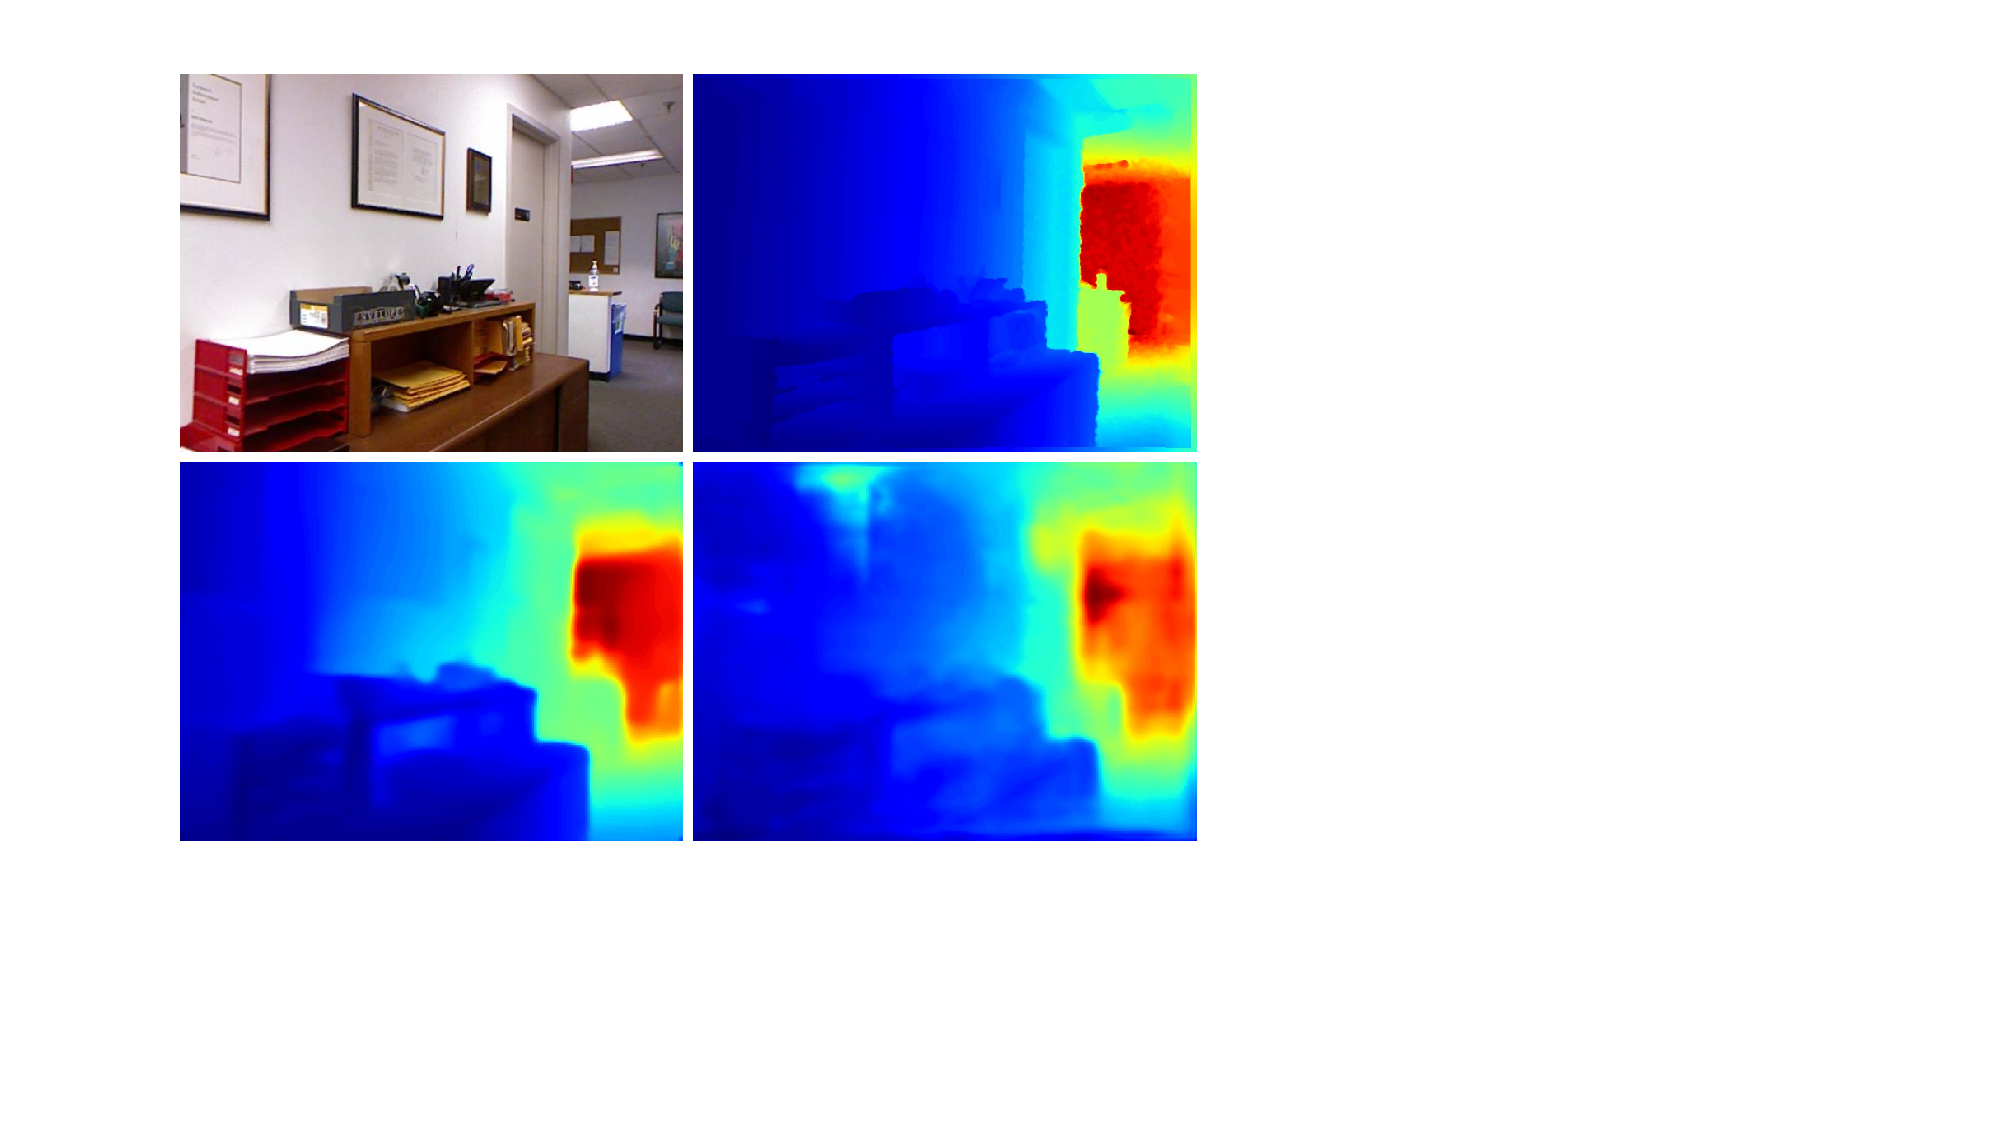
\includegraphics[width=0.55\linewidth]{images/nyu_class_fail.pdf}}
  \hspace{0.5cm}
  \subfigure[]
  {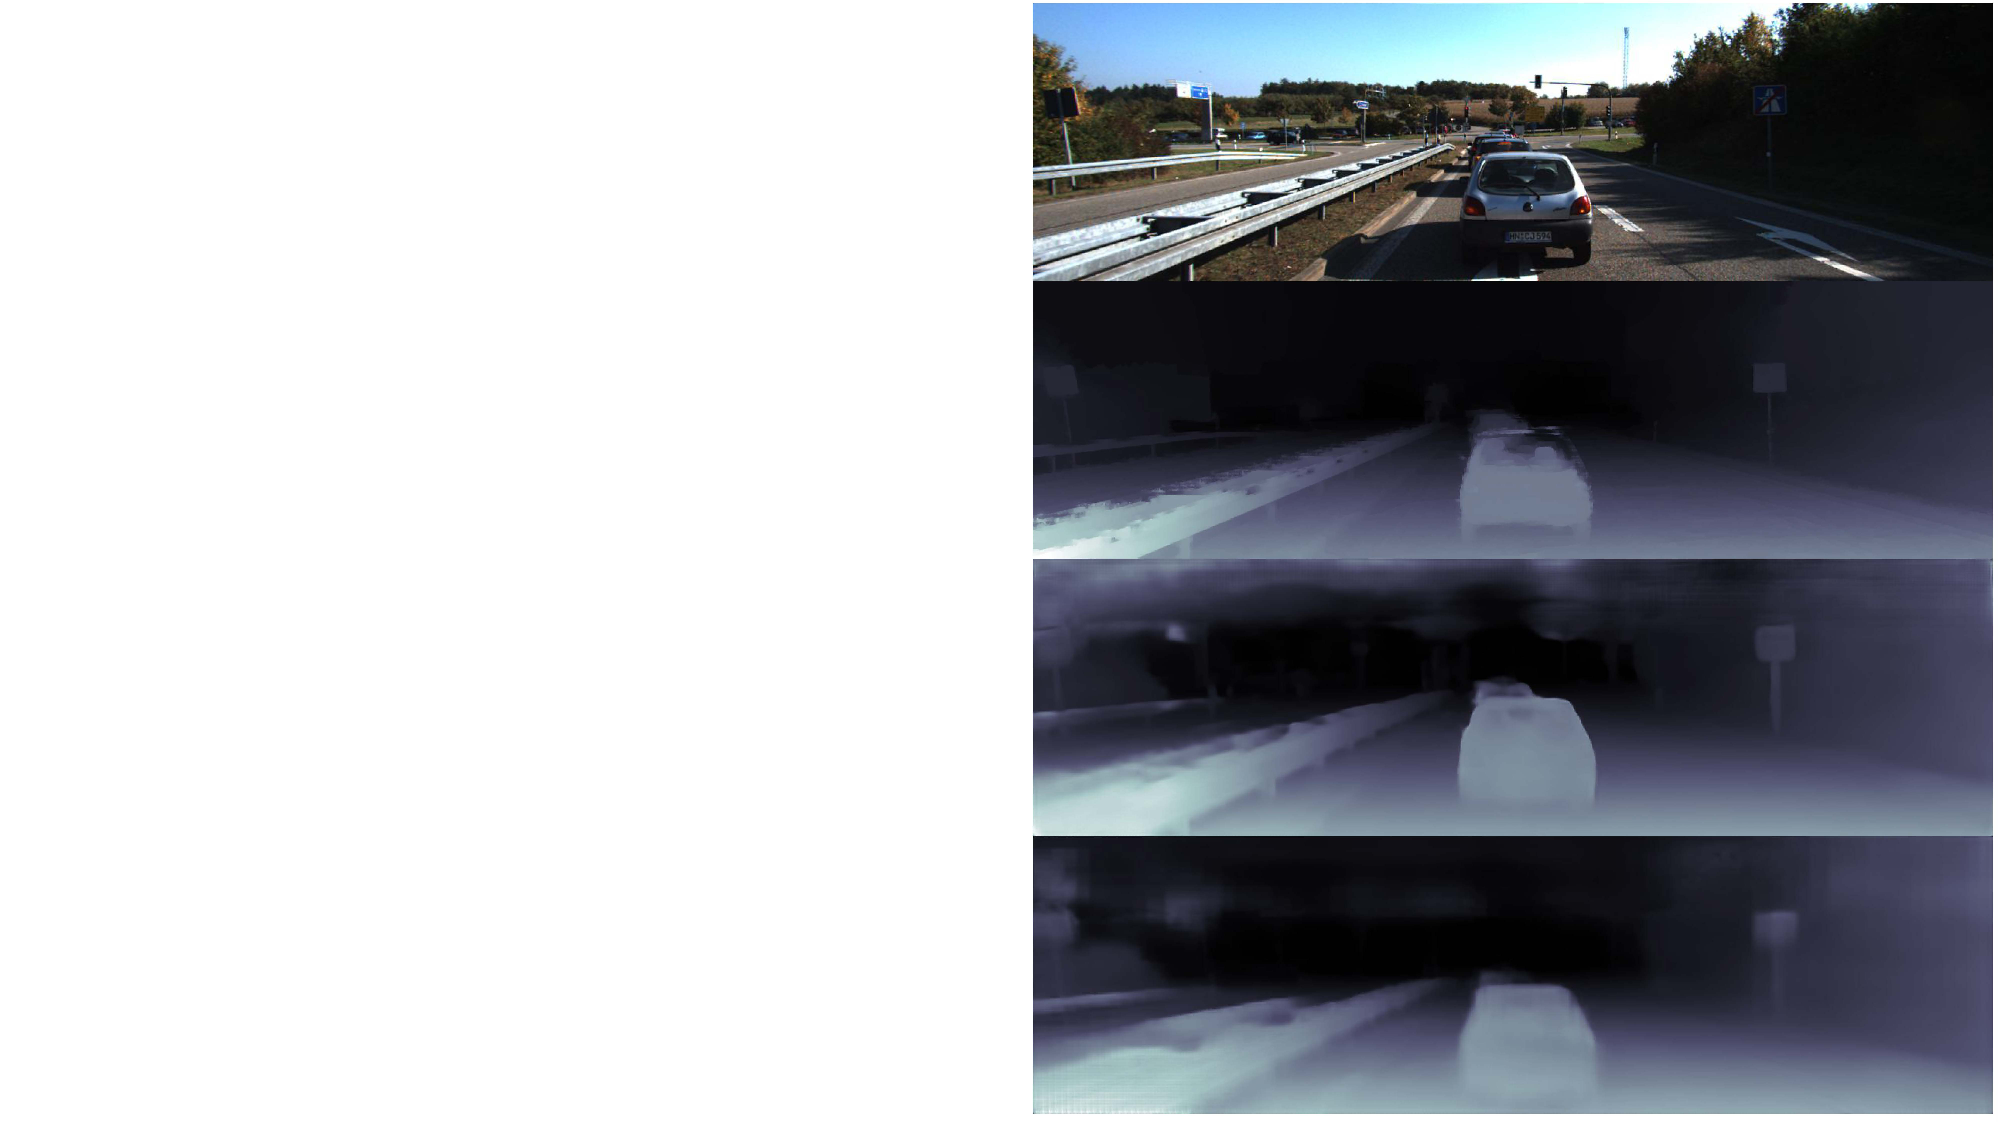
\includegraphics[width = 0.36\linewidth]{images/kitti_bts_fail.pdf}}
  \caption{
  Performance of monocular depth estimation network trained on single dataset or combined dataset. In (a), on the left top is the RGB image in NYU v2~\cite{Silberman:ECCV12}, on the right top is the ground truth depth, on the left bottom is the depth estimated by~\cite{DABC} trained on KITTI~\cite{geiger2013vision}, on the right bottom is the depth estimated by trained on NYU v2 and KITTI. In (b), from top to bottom are the RGB image of KITTI, ground truth depth, the depth estimated by~\cite{bts} trained on NYU v2, and depth estimated by~\cite{bts} trained on NYU v2 and KITTI.}
\label{train_once_problem}
\end{figure}

With the rapid development of Convolutional Neural Network (CNN) and the advance of tremendous data, it is possible for a deep network to learn this unconstrained mapping from a single 2D image to its corresponding depth. Since Saxena \textit{et al.}~\cite{saxena2006learning} creatively applied CNN to depth estimation, learning-based methods have been fully exploited to estimate depth~\cite{FuCVPR18-DORN,godard2017unsupervised,Godard_2019_ICCV,lee2019monocular,zhou2017unsupervised,eigen2014depth,bts,xu2018structured}, including supervised, semi-supervised, and unsupervised estimation. Although previous works have achieved remarkable performance, most of them are trained and evaluated on only one single dataset with one specific data distribution. It means that the generalization ability of monocular depth estimation has not been explored yet. Referring to Fig.~\ref{train_once_problem}, monocular depth estimation networks trained on outdoor scenes achieve impressive performance on outdoor scenes but poor performance on indoor scenes, vice versa. Moreover, when trained on the combined dataset (NYU v2 ~\cite{Silberman:ECCV12} plus KITTI~\cite{geiger2013vision}), the performance of current monocular depth estimation methods on the single dataset jumps off a cliff. It means current monocular depth estimation methods are not good at learning a mapping that can be applied to both indoor and outdoor scenes.

To this end, we try to learn a single monocular depth estimation network based on self-distillation to adapt two totally different scenes simultaneously, e.g., indoor and outdoor. The pipeline of our proposed method is shown in Fig.~\ref{Stream of algorithm}. Specifically, we utilize two student encoders to extract representation features from 2D images of two different datasets, respectively. Note that these two student encoders share the same set of weights. After the feature extraction, we introduce a dissimilarity loss to penalize the similarity between features of two different datasets. Finally, we adopt a decoder to estimate the final depth from encoded features, which is supervised by corresponding ground truth depth. The whole learning pipeline is conducted in an end-to-end way.

The contributions of this work are summarized as follows:
\begin{itemize}
  \item We propose a novel self-distillation framework for monocular depth estimation.
  \item To our best knowledge, we are the first to explore the generalization ability of monocular depth estimation network across datasets of different scenes, e.g., indoor and outdoor.  
  \item Comprehensive experiments demonstrate that our proposed method achieves a leading performance among other state-of-the-art monocular depth estimation methods.
\end{itemize}

\section{Related Work}
In this paper, self-distillation is used to solve the generalization 
problem of monocular depth estimation in indoor and outdoor scenes,
thus we review the development of monocular depth estimation and
knowledge distillation in this section.

\subsection{Monocular depth estimation}
Depth Estimation, which is essential for understanding 3D
scenes, has been a research focus for years. Earlier works
can be generally classified into two groups:
sensor-based~\cite{zhang2012microsoft,yoneda2014lidar} and geometry-based~\cite{zou2010method,cao2015summary,ullman1979interpretation} methods. Thanks to the leading performance achieved by Krizhevsky \emph{et al.}~\cite{10.1145/3065386}, CNN has 
demonstrated its outstanding ability in image processing then
learning-based methods 
began to prosper. In this subsection we focus on the learning-based
methods.

\textbf{Supervised methods} first appeared and achieved remarkable results. Saxena \emph{et al.}~\cite{saxena2006learning} employed Markov Random Field (MRF) to fit the mapping from features to depth. Eigen \emph{et al.}~\cite{eigen2014depth} expolited a two stages network to
generate depth maps from coarse to fine. The same team~\cite{7410661} proposed a model addressed three differnet tasks, normal prediction, semastic segmentation and MDE. Liu \textit{et al.}~\cite{liu2015deep} integrate CNN and continuous Conditional Random Field~(CRF) to predict depth value from a monocular image. 
liu \emph{et al.}~\cite{liu2015learning} further present an effective model and a novel superpixel pooling method. Li \emph{et al.}~\cite{li2015depth} first employed CNN to regress the depth in super-pixel scale, then post-processed the depth with CRF. Laina \emph{et al.}~\cite{laina2016deeper} proposed a fully convolutional residual architecture optimized by a novel reverse Hber loss. Cao \emph{et al.}~\cite{cao2017estimating} address MDE as a classification problem on piexel level, a deep residual network is proposed supervised by class labels discretized from ground truth depth values. \cite{2015semantic,2016semantic}  jointly train depth estimation network and semantic network exploit the information related to two tasks. Relative depth information is used in monocular depth estimation. Chen~\cite{NIPS2016_0deb1c54} proposed a relative depth dataset. Lee \textit{et al.}~\cite{lee2019monocular} estimate relative depths and ordinary depths with CNN.

\textbf{Unsupervised methods}~\cite{godard2017unsupervised,Godard_2019_ICCV,zhou2017unsupervised} emerged since the need of vast amounts of ground truth to train a network has been a weekness for supervised methods. Garg \emph{et al.}~\cite{garg2016unsupervised} constructed a CNN to generate a depth map for the source image and exploit it to synthesis a fake target image, photometric error as the loss function optimize the CNN constantly. Godard \textit{et al.}~\cite{godard2017unsupervised} predict the disparity map in a unsupervised manner use a network constrained with left-right consistency. In their subsequent work~\cite{Godard_2019_ICCV} occlusion, camera motion problem are settled, which makes an impressive improvement. Kuznietsov \textit{et al.}~\cite{Kuznietsov2017} proposed a semi-supervised method combining a model supervised only by sparse depth labels with a unsupervised model. Chen \emph{et al.}~\cite{2019semantic} use semantic information for constraining the classes consistency in a stereo image pair.
\subsection{Knowledge distillation}
We also give a brief introduce about \textbf{knowledge distillation}, by which our
work is inspired.
Knowledge distillation is proposed in~\cite{hinton2015distilling}, Hinton \textit{et al.} designed a `teacher' model to import dark knowledge to the `student' encoder, which is much more light compared with the `teacher' encoder, so as to get one lightweight network. Romero \textit{et al.}~\cite{romero2014fitnets} manifested that the intermediate representations can guide the `student' improve their performances. Anil \textit{et al.}~\cite{anil2018large} proposed online distillation, in which the `teacher' and `student' update at the same time and in a end to end manner. Zhang \textit{et al.}~\cite{zhang_self_distillation} proposed self-distillation, in this frame work dark knowldege are import between two 
shared weights network, `student' learn knowledge by itself. 
\begin{figure*}[t]
  \centering
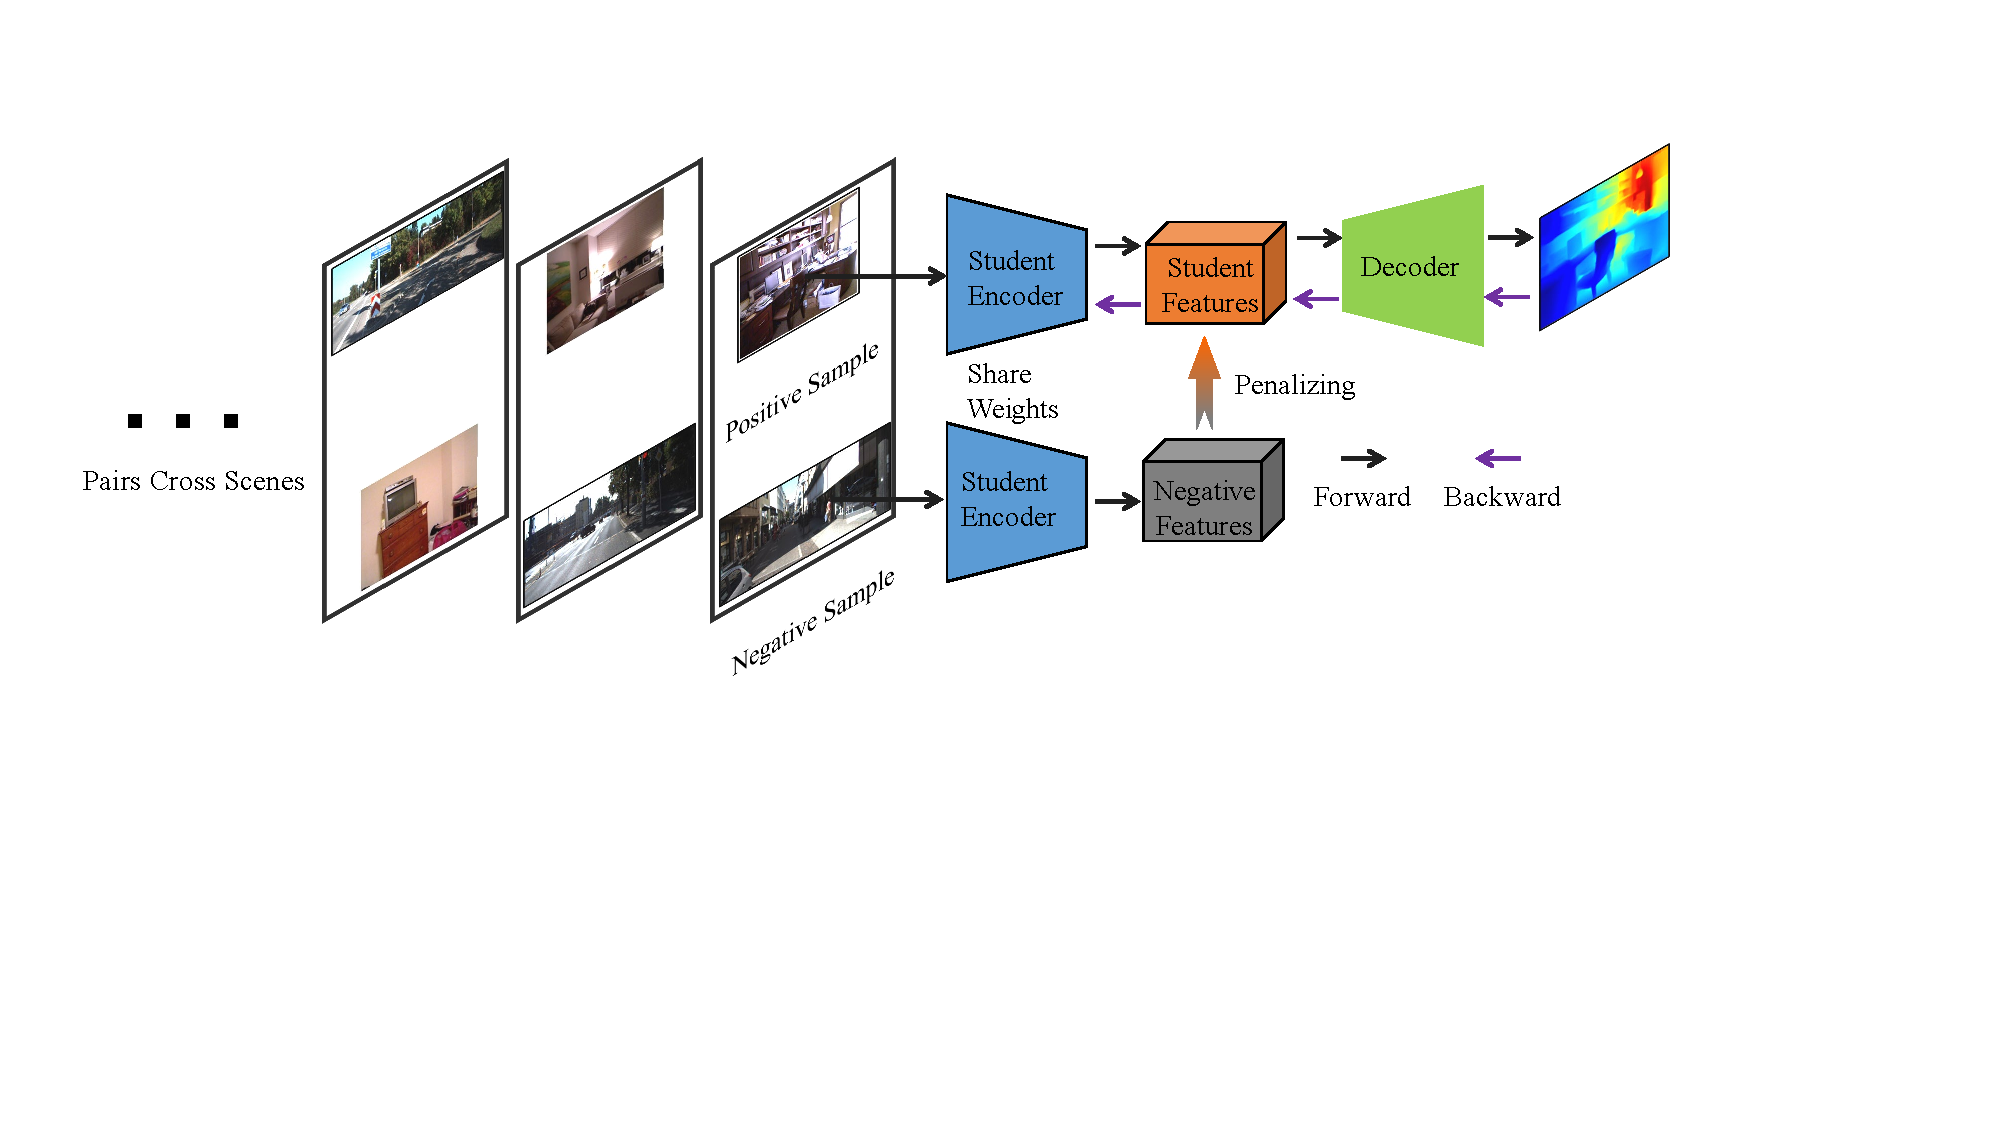
\includegraphics[width=0.9\linewidth]{images/Stream.pdf}
\centering
     \caption{Pipeline of our proposed self-distillation network for indoor and outdoor monocular depth estimation.}
 \label{Stream of algorithm} 
\end{figure*}

\section{Method}
\subsection{Problem statement}
As stated in the introduction, one single model can not fit both indoor and outdoor
scenes well. Given a training set $\mathcal{T} = \{I,D\}$, $I\in \mathcal{I}$, $D\in \mathcal{D}$, where $\mathcal{I}$ 
and $\mathcal{D}$ are the sets of RGB images and ground truth depth maps,  respectively, we look forward to
learning this ambiguous mapping $\varPhi:\mathcal{I}\rightarrow \mathcal{D}$. Faced with a training set 
with very different distributions $\mathcal{T_{IO}} = \{(I_{in},I_{out}), (D_{in},D_{out})\}$, where $I/D_{in}$ and $I/D_{out}$ are indoor and outdoor samples
respectively, a mapping with more expressiveness is required.

\subsection{Framework}
Firstly we organize two depth estimation datasets
into one dataset, which consists of both indoor and
outdoor scenes. We use this dataset with more widely distributed data 
so that an algorithm 
could work in more situations.
Instead of simply training the model with the combined dataset, we design a distillation model shown in Fig.~\ref{Stream of algorithm}. The student encoder as a feature extractor produce dense
features, which is penalized by the negative features. With the 
guidance of penalizing, the $\mathbf{X_{IO}}$ are diveded in two parts:
$\mathbf{X_{IO}} = \{\mathbf{X_{in}},\mathbf{X_{out}}\}$, where $\mathbf{X_{IO}}$ indicates the set of feature maps containing both indoor 
and outdoor scenes.

We adopt BTS~\cite{bts} to build our encoder and decoder, which is one of the state-of-the-art MDE works. In the encoder, the spatial resolution are reduced by the repeated strided convolutional layer. In the recovering stage from 
feature maps to original resolution depth estimation, it 
utilizes the novel local planar guidance layers. This local
planar assumpation
makes the reconstruction more efficient, since the layer
learns only four parameters instead of $k^2$ for a $\textbf{H}/k\times\textbf{W}/k$ feature maps if adopting traditional deconvolution.
%Relying on this innovation, this method
%achieved remarkable result as shown in 
%Table~\ref{tab:nyu quantitative result} and 
%Table~\ref{tab:kitti quantitative result}.
 
To obtain two feature maps with the same size, we design an
adaptive-pooling layer behind the feature extract module,
KITTI and NYU v2 feature maps size become $44\times88$
and $52\times68$ through the feature extractor, then we 
unify them to $44\times68$ by this adaptive-pooling layer.
%(multiple means two here specially since we want our 
%subdatasets 
%contain same quality level images,so we discard
%Make3D~\cite{Make3D},
%which contains
%534 images and its images are too little to compare
%with KITTI~\cite{geiger2013vision} and NYU depth v2~\cite{Silberman:ECCV12}) at once with a semi-supervised way.

\begin{algorithm*}[tbh]
  \caption{Self-Distillation train procedure of Indoor-Outdoor Depth Estimation}
  \KwSty{Parameters to be trained:}

      Initialize KITTI Parameter: $\alpha$,
      NYU Parameter: $\beta$.
      
      \While{ $\alpha$ or $\beta$ has not converged} 
      {Randomly sample a batch of KITTI or NYU images

        \If(){KITTI Batch sampled}{
          Sample a NYU batch simultaneously.\\
        \KwIn{KITTI-batch are fed to student encoder.}
        Update $\alpha$ by optimize the loss $\mathcal{L}_{scale-invariant}$.\\
        \KwIn{NYU-batch are fed to negative student encoder.}
        Pull apart the distance from $\beta$ to $\alpha$ by optimize the loss $\mathcal{L}_{dissimilarity}$.
        }
        \If(){NYU Batch sampled}{
          Sample a KITTI batch simultaneously.\\
        \KwIn{NYU-batch are fed to student encoder.}
        Update $\alpha$ by optimize the loss $\mathcal{L}_{scale-invariant}$.\\
        \KwIn{KITTI-batch are fed to negative student encoder.}
        Pull apart the distance from $\alpha$ to $\beta$ by optimize the loss$\mathcal{L}_{dissimilarity}$.
        }
      }
  \label{alg:backbone_alg}
  \end{algorithm*}

\subsection{Loss functions}
On the one hand, we need to make the network fit two
datasets, on the other hand, we need the network to
distinguish  two different datasets, so we design
two loss functions. Therefore, the total loss function is
weighted linearly by these sub-loss function terms.

The student encoder which is responsible for narrowing the gap within the
category of datasets, are constrained with the 
scale-invariant error loss function in \cite{eigen2014depth}:
\begin{align}
  \mathcal{L}_{scale-invariant} = \frac{1}{N}\sum_{i}g_i^2-\frac{\lambda}{N^2}(\sum_{i}g_i)^2
\end{align}
where $g_i=\log d_i^*-\log d_i$, $d_i^*$ and $d_i$ stand for ground truth depth, 
predicted depth respectively, $N$
denotes the total number of pixels. Finally we adopt
the loss in \cite{bts} since properly scaling the range of the loss could improve the performance:
\begin{align}
 \mathcal{L}_{scale-invariant} = \alpha\sqrt{\frac{1}{N}\sum_{i}g_i^2-\frac{\lambda}{N^2}(\sum_{i}g_i)^2} 
\end{align}
$\alpha$ is set to 10 in all experinments.

If a network has more expressiveness 
it can generate specific depth map according
to different scenes. So we design $\mathcal{L}_
{dissimilarity}$ to distinguish
between different data sets.
The negative student encoder share weights 
with the students encoder. It calculates negative feature maps with a batch of
contrary data, which are used to expand the gap out of the category of datasets. 
The cosine similarity loss pull apart the relevance of these two
feature maps: 
\begin{align}
  \mathcal{L}_{dissimilarity}=max(0,cos(\mathbf{x_f}, \mathbf{x_{nf}}) - margin)
\end{align} 
Where $margin$ is a coefficient and set to 0 in experiments. $\mathbf{x_{f}}$ and $\mathbf{x_{nf}}$ stand for features produced by the student encoder and negative features produced by the negative student encoder,
$cos(\mathbf{x_f}, \mathbf{x_{nf}})$ denotes the cosine of $\mathbf{x_{f}}$ and $\mathbf{x_{nf}}$, we use vectors in the channel dimension to do cosine similarity calculations. Through the penalty mechanism of this loss function, the student network can generate specific feature graphs when  different scenes are fed. 

The total loss function is organized as follows:
\begin{align}
\mathcal{L} = \gamma\mathcal{L}_{scale-invariant} + \delta\mathcal{L}_{dissimilary}
\end{align}
 $\gamma$ and $\delta$ are coefficients of these two loss. 

\section{Experiments}
In this section we conduct several experiments to illustrate the improvement
brought by our approach.
\subsection{Dataset}
Monocular depth estimation algorithms are expected to be more robust in both 
indoor and outdoor environments. However, the proposed method focus each of the them
once a time: most of previous methods are trained with a dataset and tested
immediately. To 
this end we organized a dataset containing more vary scenes, which challenges the 
generalization capacity of existing methods, since they are supposed to
fit a more complicated distribution. The NYU depth v2 and KITTI are used to
compose our dataset, they are widely used by monocular depth estimation in indoor
and outdoor respectively.

\noindent \textbf{NYU depth v2}
The NYU depth v2 dataset consists 464 indoor scenes video captured by a Microsoft
Kinect camera, which ranges from 0m to 10m. According to \cite{eigen2014depth}
we select about 17k images from 249 training scenes to compose the
proposed dataset. Note that we still use the official labeled test set containing
694 images to evaluate.
To accelerate the train progress the 
image and depth map pairs are croped to size 
of 416×544.

\noindent \textbf{KITTI}
The KITTI dataset has several subsets for different sub-tasks for autonomous
driving task. The depth maps and images are sampled by a LIDAR sensor and a camera 
equipped on a moving vehicle respectively. We follow the prior works and use
22600 images to compose our dataset. The images and depth maps 
are croped to 352×704 and then fed into the model.

\subsection{Evaluation metrics}
There are five metrics, which are widely used in MDE prior works and set a benchmark for monocular depth estimation, proposed in~\cite{eigen2014depth}:
\begin{align}
 RMSE=\sqrt{\frac{1}{\lvert N \rvert} \sum\nolimits_{i\in N}\lvert|d_i - d_i^*\rvert|^2} 
\end{align}
\begin{align}
  RMSE \ log = \sqrt{\frac{1}{\lvert N \rvert}\sum\nolimits_{i\in N}\lvert| \lg(d_i) - \lg(d_i^*) \rvert|^2}
\end{align}
\begin{align}
  Abs \ Rel=\frac{1}{\lvert N \rvert}\sum\nolimits_{i \in N}\frac{\lvert d_i - d_i^* \rvert}{d_i^*}
\end{align}
\begin{align}
  Sq \ Rel=\frac{1}{\lvert N \rvert}\sum\nolimits_{i \in N}\frac{\lvert| d_i - d_i^* \rvert|^2}{d_i^*}
\end{align}
\begin{align}
  Accuracies:\% \ of \ d_i \ s.t. \max(\frac{d_i}{d_i^*},\frac{d_i^*}{d_i})=\delta < thr 
\end{align}
Where $d_i$ and $d_i^*$ stand for predicted depth value and ground truth depth value respectively. $N$ is the total number of pixels, and $thr$ denotes three threshold $1.25$, $1.25^2$, $1.25^3$. 

\subsection{Implemention details}
\begin{figure*}[t]
  \centering
  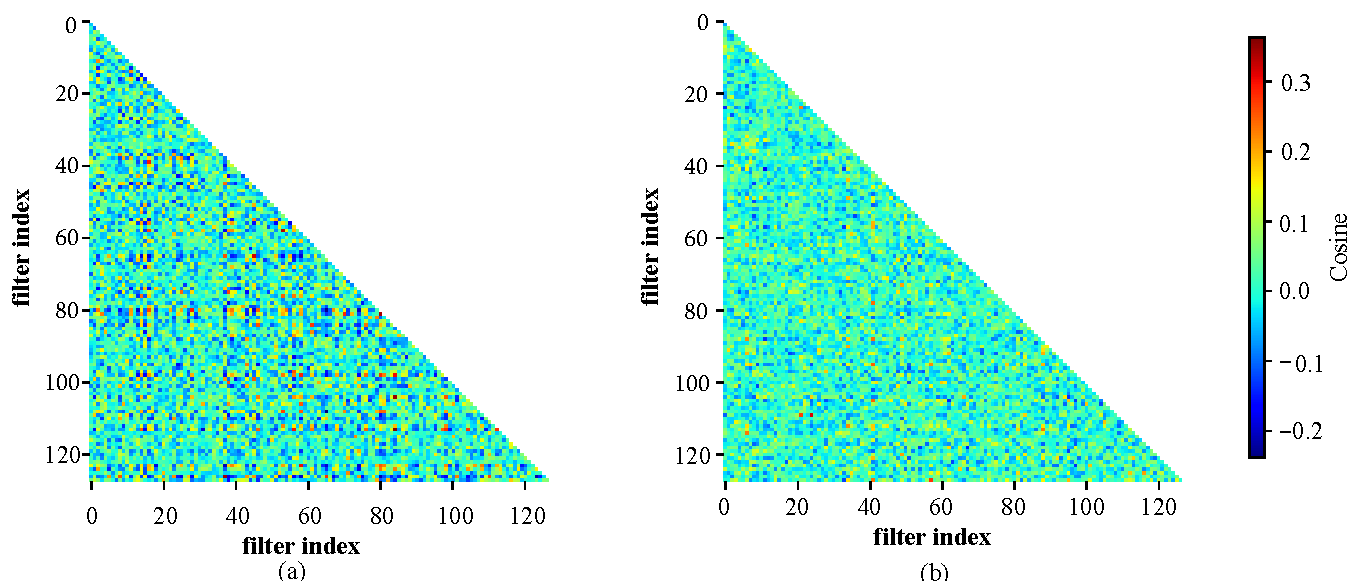
\includegraphics[width=0.85\linewidth]{images/conv_co.pdf}
  \caption{Cosine similarity comparison of filters from the last layer of the 
  encoder, (a) simply trained on a combined dataset by BTS~\cite{bts}, (b) trained in our 
  self-distillation way. The more green, the less correlation.}
  \label{fig:conv_co}
  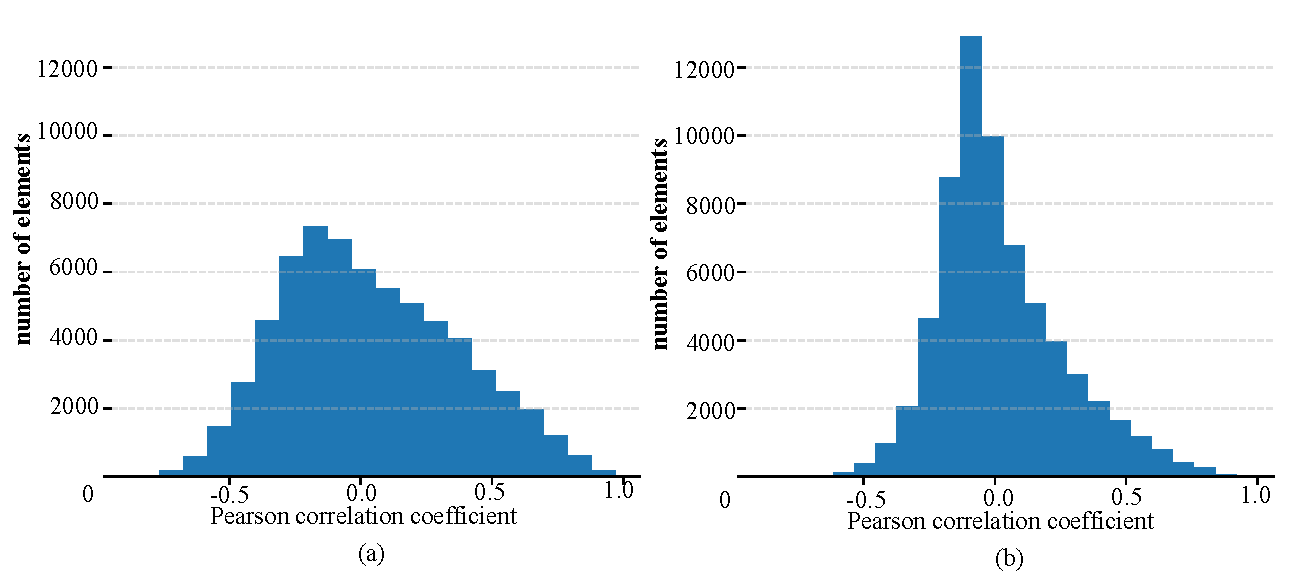
\includegraphics[width=0.85\linewidth]{images/fea_co.pdf}
  \caption{Statistical histogram of pearson correlation coeficient between the each
  channel of feature maps, (a) is derived from the feature maps generated by endocer of BTS~\cite{bts}, (b) is from ours.}
  \label{fig:fea_co}
\end{figure*}
All our experiments are conducted with batch size of 4 for 80000 iterations. Since a batch of NYU images and a batch of KITTI images are poped by dataloader in one batch at the same time, we pad the NYU batch on the left, and the KITTI batch on the top, so each of them are fixed to 416 ×704, then slice them to the previous size before they are fed into the network. All data is augmentated as the same as the original work BTS~\cite{bts}, in which contrast, brightness, and color adjustment in a range of [0.9,1.1] is applied. Also the random rotation with different ranges [-1,1] and [-2.5,2.5] for NYU v2 and KITTI is preproceded respectively. We implement our self-distillation network with PyTorch~\cite{paszke2019pytorch}.
\vspace{-1cm}
\subsection{Quantitative result}
We evaluate our model on the testing sets of KITTI and NYU v2 
using Eigen split. Note that we train on combined dataset once 
but evaluate the two datasets separately. We list several 
milestone
methods in Table~\ref{tab:nyu quantitative result} and
Table~\ref{tab:kitti quantitative result}. We train~\cite{DABC} and~\cite{bts}
on KITTI and NYU v2, no matter on KITTI or NYU v2, the indicators 
declined to varying degrees when evaluate separately. This proves again the
shortcoming of ordinary networks in the face of large differences in diversity
distribution. Although most of the indicators does not recover to the level of
training with one data set, they both attenuate the decline of training both
datasets at the same time. On KITTI dataset, the $\delta<1.25^3$ metric
reaches back to its original level. Our method even performs better than original on $RMSE$ metric in Table~\ref{tab:nyu quantitative result}.
\subsection{Visualization results}
\begin{figure*}[t]
  \centering
  \subfigure[RGB Image]{
  \begin{minipage}[b]{0.15\linewidth}
  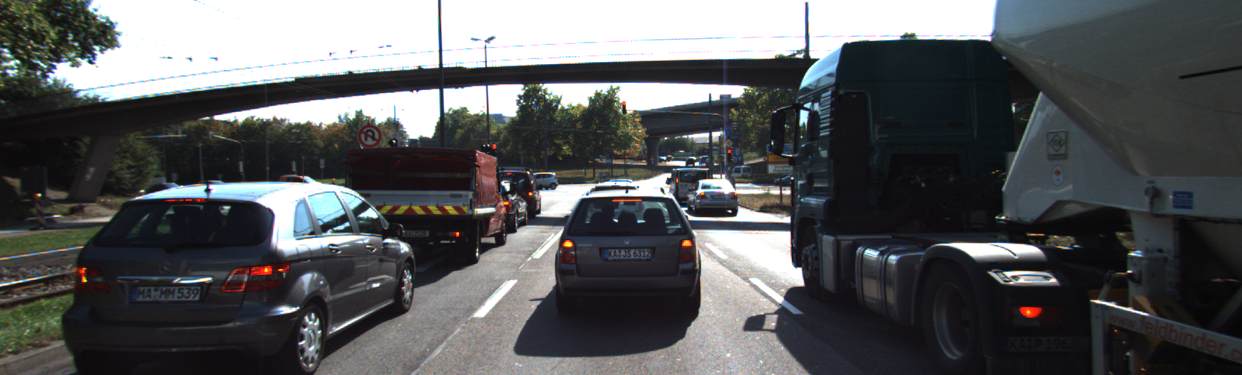
\includegraphics[width=1\linewidth]{images/kitti_rgb/0000000000.png}\vspace{4pt}
  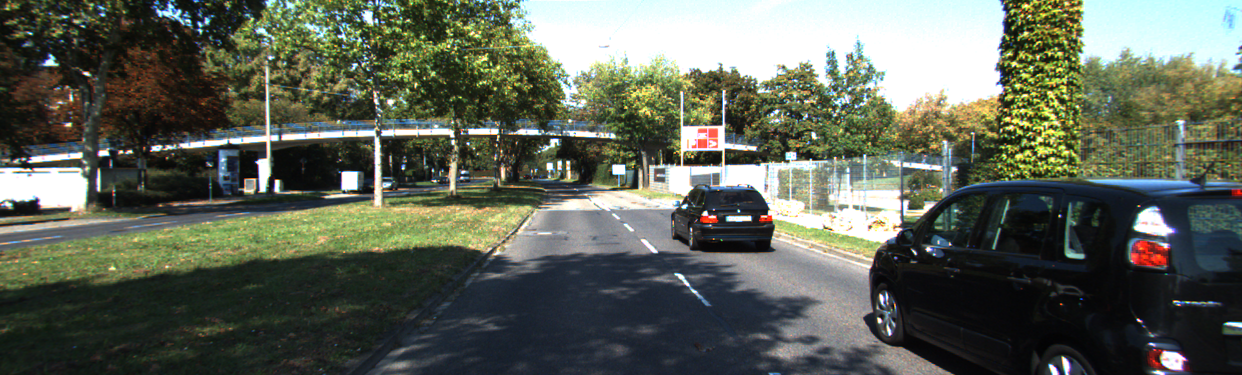
\includegraphics[width=1\linewidth]{images/kitti_rgb/0000000035.png}\vspace{4pt}
  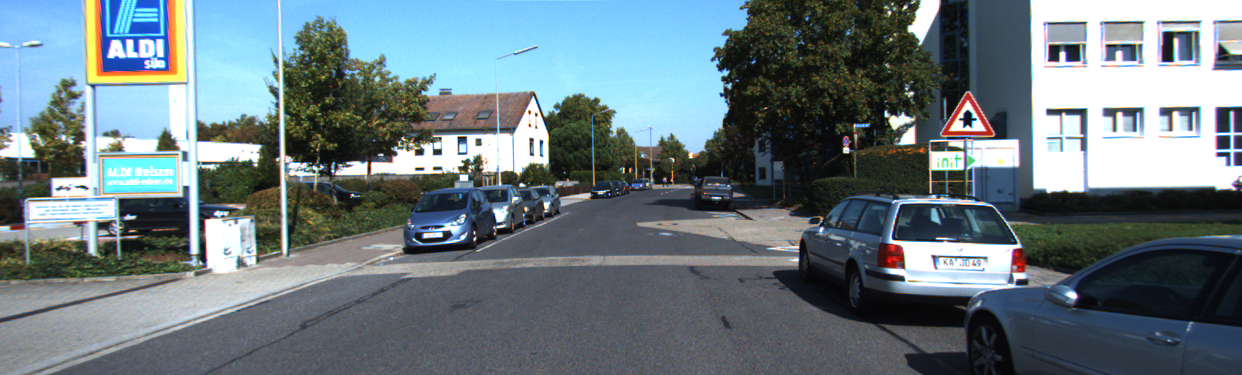
\includegraphics[width=1\linewidth]{images/kitti_rgb/0000000260.png}\vspace{4pt}
  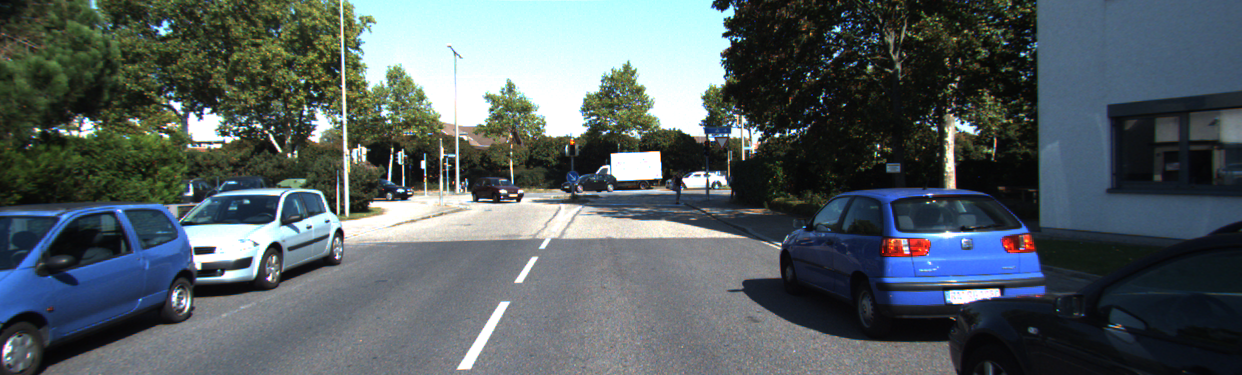
\includegraphics[width=1\linewidth]{images/kitti_rgb/0000000340.png}\vspace{4pt}
  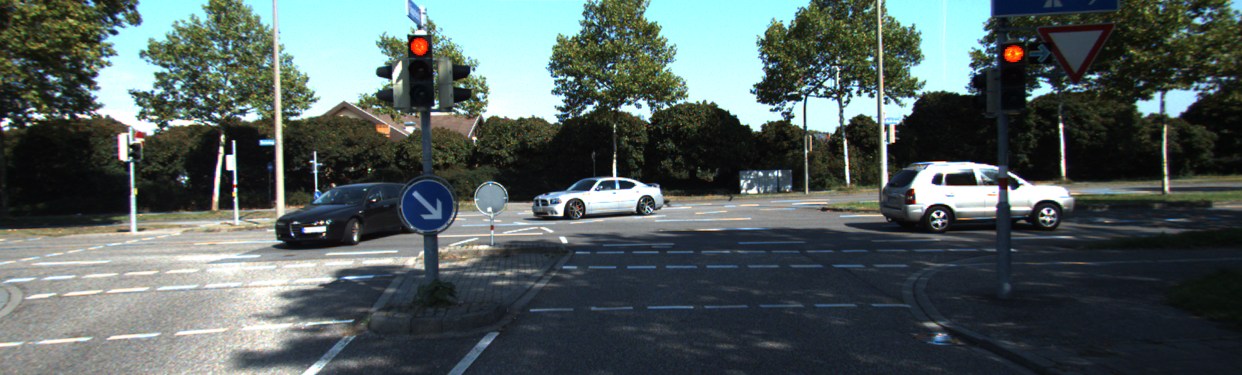
\includegraphics[width=1\linewidth]{images/kitti_rgb/0000000388.png}\vspace{4pt}
  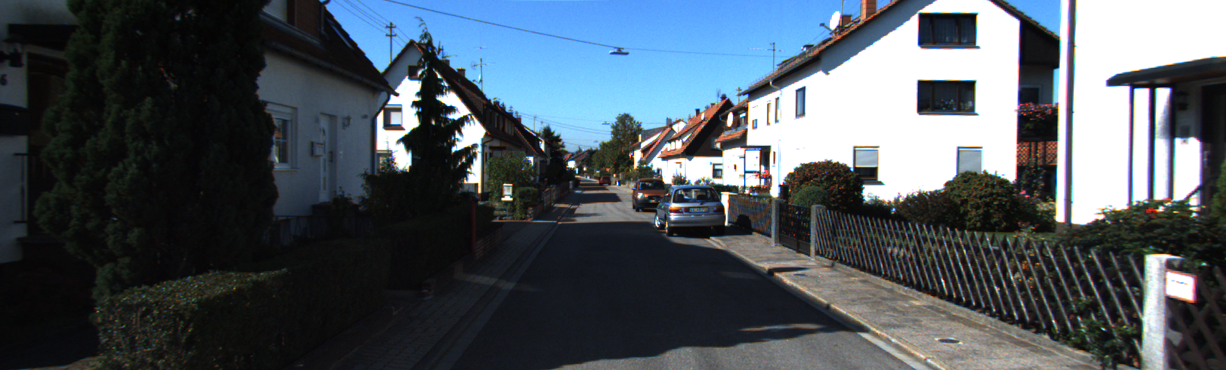
\includegraphics[width=1\linewidth]{images/kitti_rgb/0000000642.png}
  \end{minipage}}
  \subfigure[GT]{
  \begin{minipage}[b]{0.15\linewidth}
  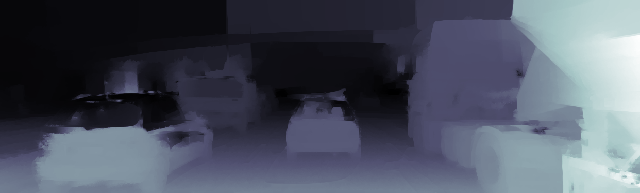
\includegraphics[width=1\linewidth]{images/kitti_gt/26_52_00.png}\vspace{4pt}
  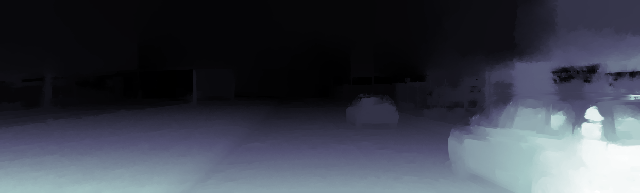
\includegraphics[width=1\linewidth]{images/kitti_gt/26_13_35.png}\vspace{4pt}
  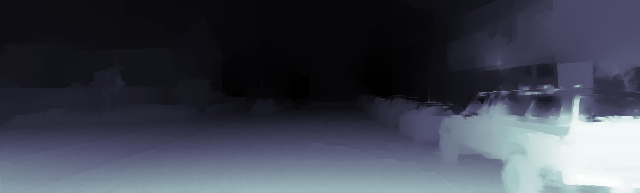
\includegraphics[width=1\linewidth]{images/kitti_gt/26_09_260.png}\vspace{4pt}
  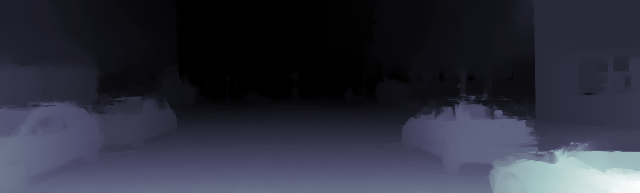
\includegraphics[width=1\linewidth]{images/kitti_gt/26_09_340.png}\vspace{4pt}
  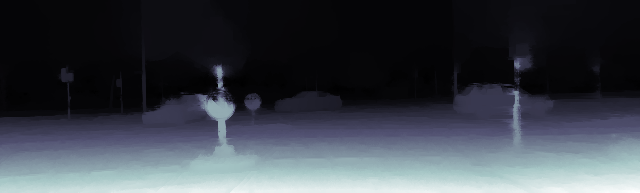
\includegraphics[width=1\linewidth]{images/kitti_gt/26_09_388.png}\vspace{4pt}
  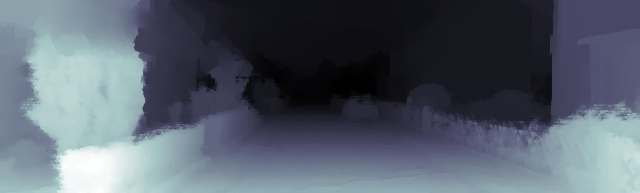
\includegraphics[width=1\linewidth]{images/kitti_gt/30_18_642.png}
  \end{minipage}}
  \subfigure[DORN~\cite{FuCVPR18-DORN}]{
  \begin{minipage}[b]{0.15\linewidth}
  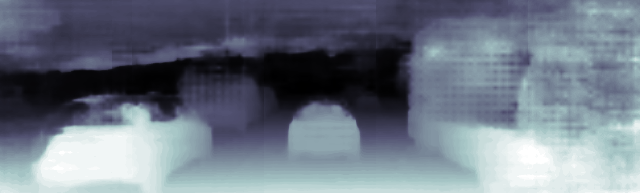
\includegraphics[width=1\linewidth]{images/dorn/2011_09_26_drive_0052_sync_0000000000.png}\vspace{4pt}
  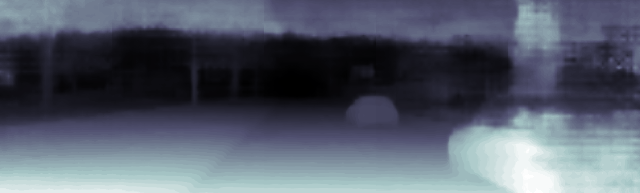
\includegraphics[width=1\linewidth]{images/dorn/2011_09_26_drive_0013_sync_0000000035.png}\vspace{4pt}
  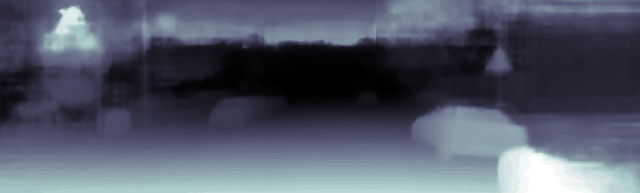
\includegraphics[width=1\linewidth]{images/dorn/2011_09_26_drive_0009_sync_0000000260.png}\vspace{4pt}
  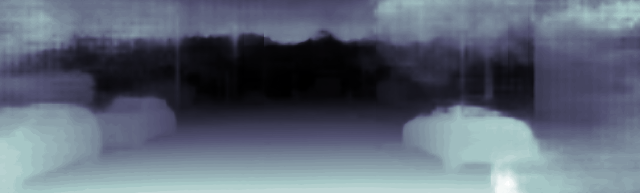
\includegraphics[width=1\linewidth]{images/dorn/2011_09_26_drive_0009_sync_0000000340.png}\vspace{4pt}
  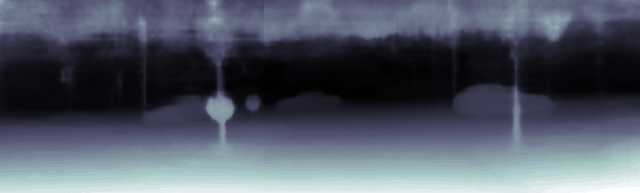
\includegraphics[width=1\linewidth]{images/dorn/2011_09_26_drive_0009_sync_0000000388.png}\vspace{4pt}
  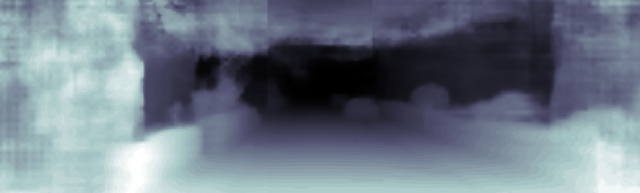
\includegraphics[width=1\linewidth]{images/dorn/2011_09_30_drive_0018_sync_0000000642.png}
  \end{minipage}}
  \subfigure[SfmLearner~\cite{zhou2017unsupervised}]{
  \begin{minipage}[b]{0.15\linewidth}
  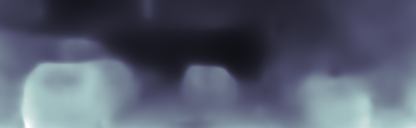
\includegraphics[width=1\linewidth]{images/kitti_sfm/2011_09_26_drive_0052_sync_0000000000.png}\vspace{3.5pt}
  
\includegraphics[width=1\linewidth]{images/kitti_sfm/2011_09_26_drive_0013_sync_0000000035.png}\vspace{3.5pt}
  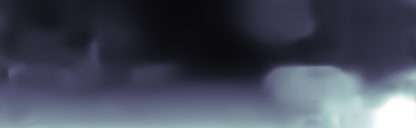
\includegraphics[width=1\linewidth]{images/kitti_sfm/2011_09_26_drive_0009_sync_0000000260.png}\vspace{3.5pt}
  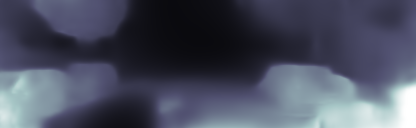
\includegraphics[width=1\linewidth]{images/kitti_sfm/2011_09_26_drive_0009_sync_0000000340.png}\vspace{3.5pt}
  
\includegraphics[width=1\linewidth]{images/kitti_sfm/2011_09_26_drive_0009_sync_0000000388.png}\vspace{3.5pt}
  
\includegraphics[width=1\linewidth]{images/kitti_sfm/2011_09_30_drive_0018_sync_0000000642.png}
  \end{minipage}}
  \subfigure[BTS~\cite{bts}]{
  \begin{minipage}[b]{0.15\linewidth}
  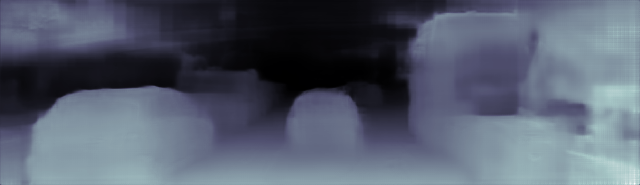
\includegraphics[width=1\linewidth]{images/kitti_without/2011_09_26_drive_0052_sync_0000000000.png}\vspace{5pt}
  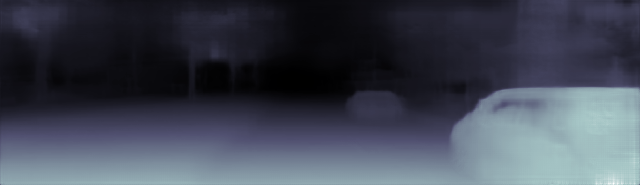
\includegraphics[width=1\linewidth]{images/kitti_without/2011_09_26_drive_0013_sync_0000000035.png}\vspace{5pt}
  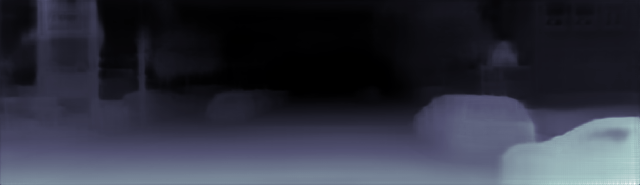
\includegraphics[width=1\linewidth]{images/kitti_without/2011_09_26_drive_0009_sync_0000000260.png}\vspace{5pt}
  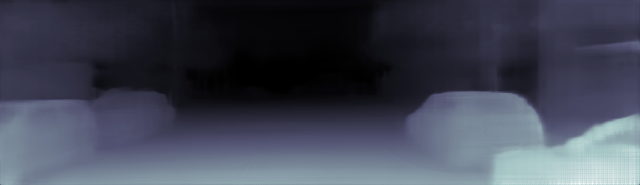
\includegraphics[width=1\linewidth]{images/kitti_without/2011_09_26_drive_0009_sync_0000000340.png}\vspace{5pt}
  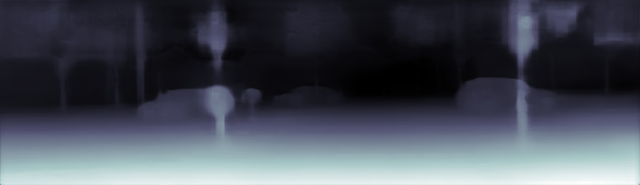
\includegraphics[width=1\linewidth]{images/kitti_without/2011_09_26_drive_0009_sync_0000000388.png}\vspace{5pt}
  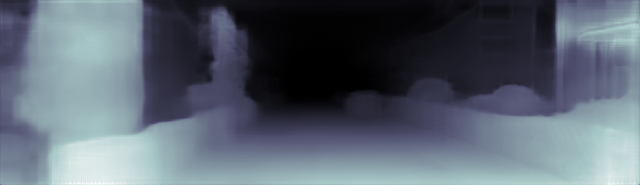
\includegraphics[width=1\linewidth]{images/kitti_without/2011_09_30_drive_0018_sync_0000000642.png}
  \end{minipage}}
  \subfigure[Ours]{
  \begin{minipage}[b]{0.15\linewidth}
  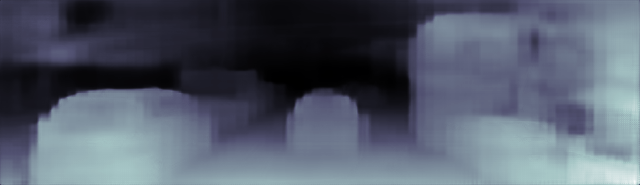
\includegraphics[width=1\linewidth]{images/kitti_result/2011_09_26_drive_0052_sync_0000000000.png}\vspace{5pt}
  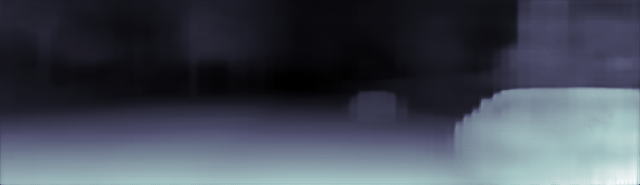
\includegraphics[width=1\linewidth]{images/kitti_result/2011_09_26_drive_0013_sync_0000000035.png}\vspace{5pt}
  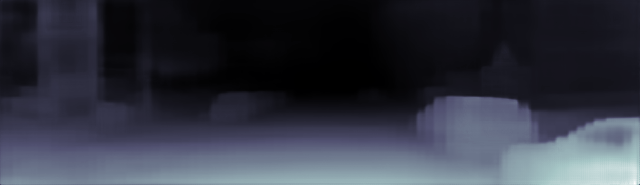
\includegraphics[width=1\linewidth]{images/kitti_result/2011_09_26_drive_0009_sync_0000000260.png}\vspace{5pt}
  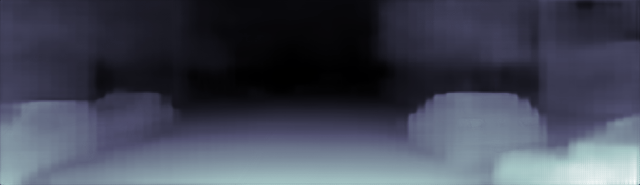
\includegraphics[width=1\linewidth]{images/kitti_result/2011_09_26_drive_0009_sync_0000000340.png}\vspace{5pt}
  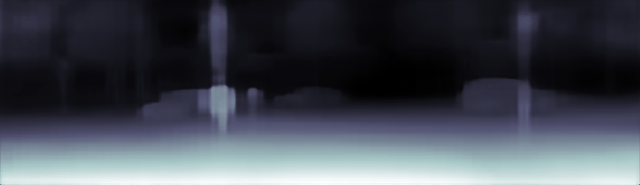
\includegraphics[width=1\linewidth]{images/kitti_result/2011_09_26_drive_0009_sync_0000000388.png}\vspace{5pt}
  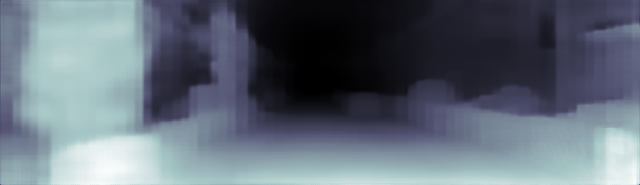
\includegraphics[width=1\linewidth]{images/kitti_result/2011_09_30_drive_0018_sync_0000000642.png}
  \end{minipage}}
  \subfigure{
    \begin{minipage}[]{0.5\linewidth}
    \centering
     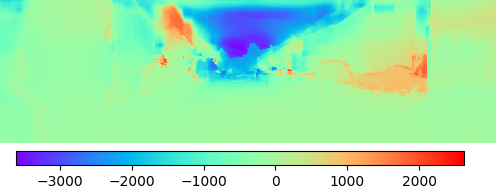
\includegraphics[width=0.95\linewidth]{images/without_error.png} 
    \end{minipage}
    \begin{minipage}[]{0.5\linewidth}
    \centering
     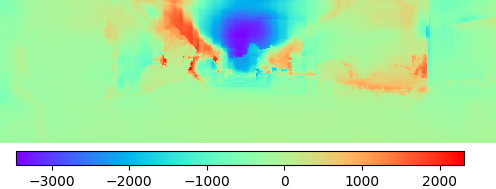
\includegraphics[width=0.95\linewidth]{images/our_error.png} 
    \end{minipage}
  }
  \caption{Visual result comparison of predicted depth map. We interpolate 
  the sparse GT maps using tool box provided on~\cite{nyu-toolbox}. Notes that the DORN~\cite{FuCVPR18-DORN} and SfmLearner~\cite{zhou2017unsupervised} are trained only on KITTI dataset, BTS~\cite{bts} and Ours are trained on two datasets. The heat maps are error maps ($map_{error} = D_{gt} - D_{pre}$) of the last depth maps predicted by BTS~\cite{bts}~(left) and ours~(right). }
  \label{KITTI visualization result}
  \end{figure*}

\begin{table*}[h]
  \centering
  \caption{Quantitative results comparisons on NYU v2 dataset.
  Best results are boldfaced.}
  \label{tab:nyu quantitative result}
  \begin{tabular}{c|cc|cccc|ccc}
    \toprule
    \multirow{2}{*}{Method} & \multicolumn{2}{c|}{Dataset}& \multicolumn{4}{c}{lower is better}&\multicolumn{3}{|c}{higher is better}\\
    &KITTI&NYU& Rel Abs & Rel Sq & RMSE& RMSE $log$ &$\delta<1.25$ &$\delta<1.25^2$ & $\delta<1.25^3$ \\   
    \midrule
    Saxena~\textit{et al.}~\cite{Make3D}&&$\surd $&0.349&-&
    1.214&-&0.447&0.745&0.897\\
    Eigen~\textit{et al.}~\cite{eigen2014depth}&&$\surd$&0.215&-
    &0.907&0.282&0.702&0.898&0.967\\
    Liu~\textit{et al.}~\cite{liu2015learning}&&$\surd$&0.213&-&0.759&-&0.650&0.906&0.976\\
    Chakrabarti~\textit{et al.}~\cite{chakrabarti2016depth}&&$\surd$&0.149&-&0.620&-&0.806&0.953&0.988\\
    Laina~\textit{et al.}~\cite{laina2016deeper}&&$\surd$&0.114&0.898&4.935&0.206&0.861&0.949&0.976\\
    Lee~\textit{et al.}~\cite{lee2019monocular}&&$\surd$&
    0.131&0.087&0.538&-&0.837&0.971&0.994\\
    Fu~\textit{et al.}~\cite{FuCVPR18-DORN}&&$\surd$&0.115&-&0.509&-&0.828&0.965&0.992\\
    Xu~\textit{et al.}~\cite{xu2018structured}&&$\surd$&0.125&-&0.593&-&0.806&0.952&0.986\\
    \hline
    Li~\textit{et al.}~\cite{DABC}&&$\surd$&0.124&&0.597&0.366&0.814&0.960&0.988\\
    Li~\textit{et al.}~\cite{DABC}&$\surd$&$\surd$&0.174&-&0.796&0.401&0.724&0.911&0.942\\
    \hline
    Lee~\textit{et al.}~\cite{bts}&&$\surd$&\textbf{0.110}&-&0.392&\textbf{0.047}&\textbf{0.885}&\textbf{0.978}&\textbf{0.994}\\
    Lee~\textit{et al.}~\cite{bts}&$\surd$&$\surd$&0.172&0.101&0.402&0.198&0.731&0.933&0.984\\
    Ours&$\surd$&$\surd$&0.163&\textbf{0.091}&\textbf{0.388}&0.190&0.746&0.941&0.987\\
    \bottomrule
  \end{tabular}
\end{table*}
\begin{figure*}[t]
  \centering
  \subfigure{
  \begin{minipage}[t]{0.15\linewidth}
  \centering
  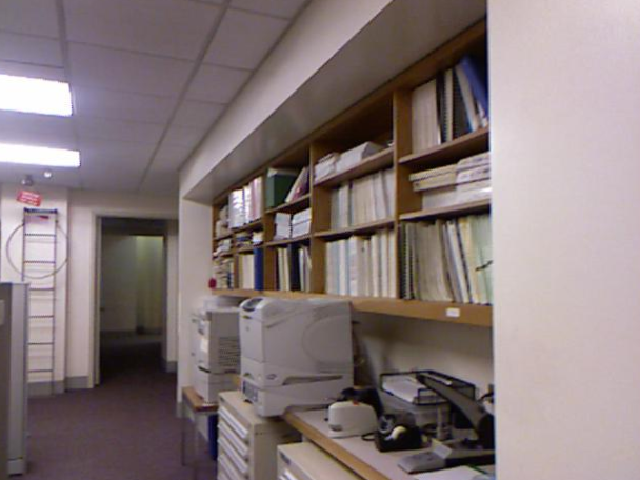
\includegraphics[width=1\linewidth]{images/nyu_rgb/15.png}
  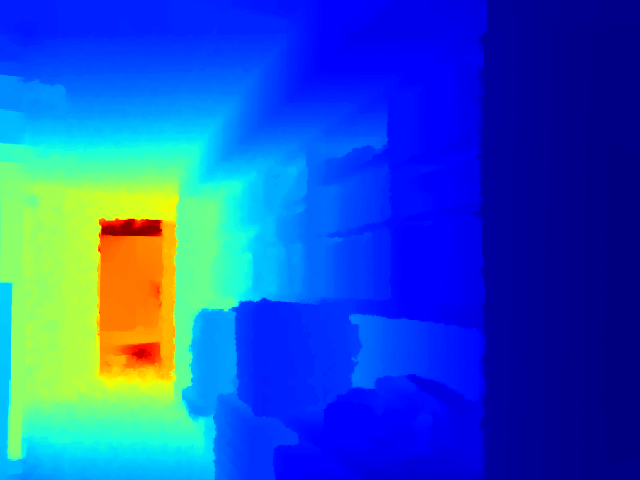
\includegraphics[width=1\linewidth]{images/nyu_gt/15.png}
  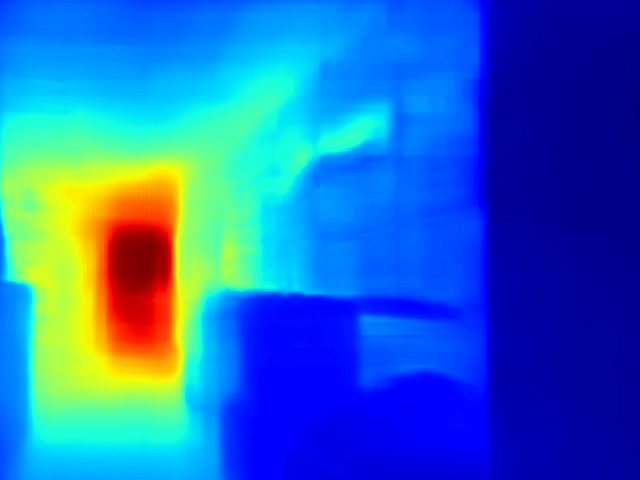
\includegraphics[width=1\linewidth]{images/nyu_result/office_rgb_00015.png}
  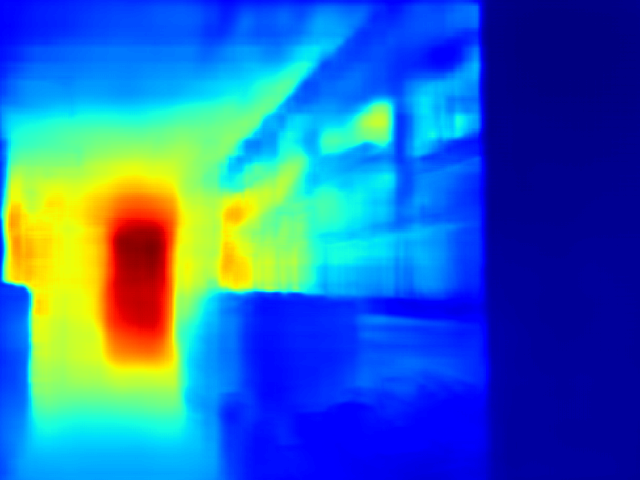
\includegraphics[width=1\linewidth]{images/nyu_without/office_rgb_00015.png}
  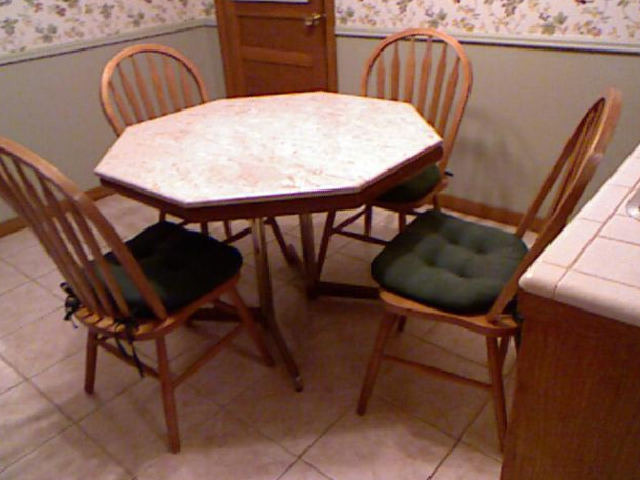
\includegraphics[width=1\linewidth]{images/nyu_rgb/760.png}
  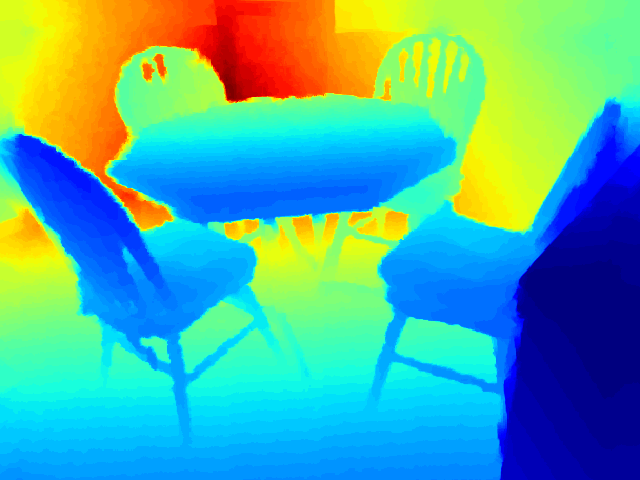
\includegraphics[width=1\linewidth]{images/nyu_gt/760.png}
  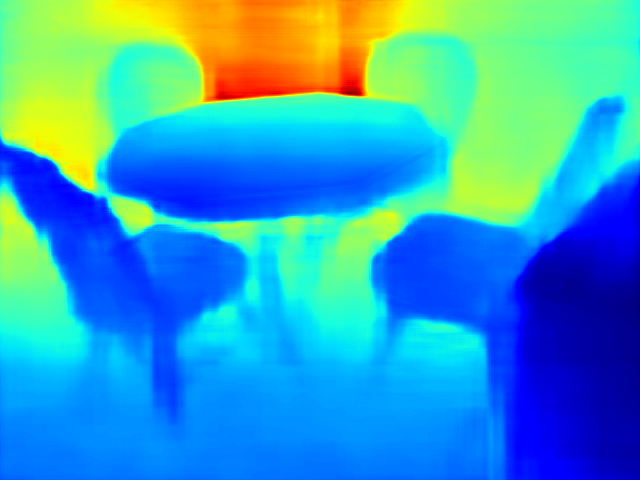
\includegraphics[width=1\linewidth]{images/nyu_result/kitchen_rgb_00760.png}
  \includegraphics[width=1\linewidth]{images/nyu_without/kitchen_rgb_00760.png}
  %\caption{fig1}
  \end{minipage}%
  }
  \subfigure{
  \begin{minipage}[t]{0.15\linewidth}
  \centering
  \includegraphics[width=1\linewidth]{images/nyu_rgb/170.png}
  \includegraphics[width=1\linewidth]{images/nyu_gt/170.png}
  \includegraphics[width=1\linewidth]{images/nyu_result/bedroom_rgb_00170.png}
  \includegraphics[width=1\linewidth]{images/nyu_without/bedroom_rgb_00170.png}
  \includegraphics[width=1\linewidth]{images/nyu_rgb/850.png}
  \includegraphics[width=1\linewidth]{images/nyu_gt/850.png}
  \includegraphics[width=1\linewidth]{images/nyu_result/kitchen_rgb_00850.png}
  \includegraphics[width=1\linewidth]{images/nyu_without/kitchen_rgb_00850.png}
  %\caption{fig2}
  \end{minipage}%
  }
  \subfigure{
  \begin{minipage}[t]{0.15\linewidth}
  \centering
  \includegraphics[width=1\linewidth]{images/nyu_rgb/431.png}
  \includegraphics[width=1\linewidth]{images/nyu_gt/431.png}
  \includegraphics[width=1\linewidth]{images/nyu_result/playroom_rgb_00431.png}
  \includegraphics[width=1\linewidth]{images/nyu_without/playroom_rgb_00431.png}
  \includegraphics[width=1\linewidth]{images/nyu_rgb/1078.png}
  \includegraphics[width=1\linewidth]{images/nyu_gt/1078.png}
  \includegraphics[width=1\linewidth]{images/nyu_result/bedroom_rgb_01078.png}
  \includegraphics[width=1\linewidth]{images/nyu_without/bedroom_rgb_01078.png}
  %\caption{fig2}
  \end{minipage}%
  }
  \subfigure{
  \begin{minipage}[t]{0.15\linewidth}
  \centering
  \includegraphics[width=1\linewidth]{images/nyu_rgb/566.png}
  \includegraphics[width=1\linewidth]{images/nyu_gt/566.png}
  \includegraphics[width=1\linewidth]{images/nyu_result/kitchen_rgb_00566.png}
  \includegraphics[width=1\linewidth]{images/nyu_without/kitchen_rgb_00566.png}
  \includegraphics[width=1\linewidth]{images/nyu_rgb/1149.png}
  \includegraphics[width=1\linewidth]{images/nyu_gt/1149.png}
  \includegraphics[width=1\linewidth]{images/nyu_result/bedroom_rgb_01149.png}
  \includegraphics[width=1\linewidth]{images/nyu_without/bedroom_rgb_01149.png}
  %\caption{fig2}
  \end{minipage}%
  }
  \subfigure{
  \begin{minipage}[t]{0.15\linewidth}
  \centering
  \includegraphics[width=1\linewidth]{images/nyu_rgb/668.png}
  \includegraphics[width=1\linewidth]{images/nyu_gt/668.png}
  \includegraphics[width=1\linewidth]{images/nyu_result/bathroom_rgb_00668.png}
  \includegraphics[width=1\linewidth]{images/nyu_without/bathroom_rgb_00668.png}
  \includegraphics[width=1\linewidth]{images/nyu_rgb/1313.png}
  \includegraphics[width=1\linewidth]{images/nyu_gt/1313.png}
  \includegraphics[width=1\linewidth]{images/nyu_result/living_room_rgb_01313.png}
  \includegraphics[width=1\linewidth]{images/nyu_without/living_room_rgb_01313.png}
  %\caption{fig2}
  \end{minipage}%
  }
  \subfigure{
  \begin{minipage}[t]{0.15\linewidth}
  \centering
  \includegraphics[width=1\linewidth]{images/nyu_rgb/706.png}
  \includegraphics[width=1\linewidth]{images/nyu_gt/706.png}
  \includegraphics[width=1\linewidth]{images/nyu_result/bathroom_rgb_00706.png}
  \includegraphics[width=1\linewidth]{images/nyu_without/bathroom_rgb_00706.png}
  \includegraphics[width=1\linewidth]{images/nyu_rgb/1399.png}
  \includegraphics[width=1\linewidth]{images/nyu_gt/1399.png}
  \includegraphics[width=1\linewidth]{images/nyu_result/dining_room_rgb_01399.png}
  \includegraphics[width=1\linewidth]{images/nyu_without/dining_room_rgb_01399.png}
  %\caption{fig2}
  \end{minipage}%
  }
  \centering
  \caption{Visual result comparison of predicted depth maps tested on NYU v2 but trained on combined dataset: RGB images~(first row), 
  ground truth~(second row), ours~(third row), BTS~\cite{bts}~(fourth row).}
  \label{nyu visualization result}
  \end{figure*}
\begin{table*}[!h]
  \centering
  \caption{Quantitative results comparisons on KITTI dataset.
  Best results are boldfaced.}
  \label{tab:kitti quantitative result}
  \begin{tabular}{c|cc|cccc|ccc}
    \toprule
    \multirow{2}{*}{Method} & \multicolumn{2}{c|}{Dataset}& \multicolumn{4}{c|}{lower is better}&\multicolumn{3}{c}{higher is better}\\
    &KITTI&NYU& Rel Abs & Rel Sq & RMSE& RMSE $log$ &$\delta<1.25$ &$\delta<1.25^2$ & $\delta<1.25^3$ \\   
    \midrule
    Saxena~\textit{et al.}~\cite{Make3D}&$\surd $&&0.280&3.012&
    8.734&0.361&0.601&0.820&0.926\\
    Eigen~\textit{et al.}~\cite{eigen2014depth}&$\surd$&&0.203&
    1.548&6.307&0.282&0.702&0.898&0.967\\
    Liu~\textit{et al.}~\cite{liu2015learning}&$\surd$&&0.201&1.584&6.471&0.273&0.680&0.898&0.967\\
    Kuznietsov~\textit{et al.}~\cite{Kuznietsov2017}&$\surd$&&0.113&0.741&4.621&0.189&0.862&0.960&0.986\\
    Godard~\textit{et al.}~\cite{godard2017unsupervised}&$\surd$&&0.114&0.898&4.935&0.206&0.861&0.949&0.976\\
    Zhow~\textit{et al.}~\cite{zhou2017unsupervised}&$\surd$&&
    0.198&1.836&6.565&0.275&0.718&0.901&0.960\\
    Fu~\textit{et al.}~\cite{FuCVPR18-DORN}&$\surd$&&0.072&0.307&\textbf{2.727}&0.120&0.932&0.984&0.994\\
    Xu~\textit{et al.}~\cite{xu2018structured}&$\surd$&&0.122&0.897&4.677&-&0.818&0.954&0.850\\
    \hline
    Li~\textit{et al.}~\cite{DABC}&$\surd$&&0.144&0.528&4.470&0.197&0.845&0.961&0.984\\
    Li~\textit{et al.}~\cite{DABC}&$\surd$&$\surd$&0.231&0.655&7.096&0.259&0.734&0.891&0.921\\
    \hline
    Lee~\textit{et al.}~\cite{bts}&$\surd$&&\textbf{0.059}&\textbf{0.245}&2.756&\textbf{0.096}&\textbf{0.956}&\textbf{0.993}&\textbf{0.998}\\
    Lee~\textit{et al.}~\cite{bts}&$\surd$&$\surd$&0.114&0.392&3.257&0.142&0.892&0.989&\textbf{0.998}\\
    Ours&$\surd$&$\surd$&0.115&0.389&3.036&0.144&0.890&0.989&\textbf{0.998}\\
    \bottomrule
  \end{tabular}
\end{table*}
A robust depth estimation algorithm is supposed to
generate corresponding depth map given an specific scene image, our method
makes the network extract different feature maps for different scens. However 
the expressiveness
ability also plays an important role 
for the network to generate specific depth map for extracted dense
feature map. We compute 
the cosine similarity of the last layer before adaptive
pooling layer, which downsample the feature maps to fixed
size. The Fig.~\ref{fig:conv_co}
demonstrates that our approach, as shown in (b), reduces the redundancy of
this 
filter. Nervertheless, filter from a network trained on a combined dataset
simply still
has a lot redundant neurous, which degrades the expressiveness capacity. We
also caculate the Pearson Correlation Coefficient~(PCC)
of the feature maps produced by the encoder by following this way: there
are 128 channels for the feature maps, they are 
flatted from the channel dimension to the last dimension,
which makes their size to $128\times \mathbf{(H\times W)}$, 
then we calculate the pearson correlation coeficient between the each channel 
of feature maps in Fig.~\ref{fig:fea_co}. Compared with the simple training with two datasets, the
PCC between each channel of the feature map generated by our
self-distillation method~(b) is more
concentrated around 0, which means that the features of the feature maps
generated by
our method have less correlation. 

We compare our method with several state-of-the-art methods in Fig.~\ref{KITTI visualization result}. Our method performs better in reconstructing boundary and
accuracy of depth map. To illustrate the perfomance improvement of our
method, we magnify the error maps of
the last depth image predicted by BTS~\cite{bts}~(left) and 
our method~(right). It can be seen that our method has a significant improvement in
long-range prediction than BTS~\cite{bts}, the far error pixels number decrease a 
lot. The NYU v2 visualization are displaced in Fig.~\ref{nyu visualization result},
 our method performs better in detail, for instance the bookcase, human body and 
 bathhub.



%%%%%%%%%%%%%%%%%%%%%%%%%%%%%%%%%%%%%%%%%%%%%%%%%%%%%%%%%%%%%%%%%%%%%%%

\section{Conclusion}
In this paper, we concern a problem that has been ignored by 
prior works, the degradation problem when a monocular depth estimation network
trained on a diversity dataset.
We proposed a self-distillation model to tackle the adaptive 
problem, it is caused by the dilemma of using one mapping to fit two totally
different distributions. On the on hand we 
designed a student encoder to learn the mapping, On the other hand, we designed a
negative student encoder to guidance the network 
distinguishes two datasets. Our experiments demonstrate that our 
method expand the expressiveness capacity of the network. We 
innovatively use the combined dataset with KITTI and NYU v2 as
diversity training dataset. Quantitative experiments show that 
our method achieves more favorable perfomance.


\begin{acknowledgements}
This work was supported by the National Natural Science Foundation of China (No. 62071500, 61701313), Open project of Guangdong Key
Laboratory of Intelligent Information Processing, Shenzhen, China,
Key-Area Research and Development Program of Guangdong
Province (2020B090921003).
\end{acknowledgements}

% Authors must disclose all relationships or interests that 
% could have direct or potential influence or impart bias on 
% the work: 
%
% \section*{Conflict of interest}
%
% The authors declare that they have no conflict of interest.


% BibTeX users please use one of
%\bibliographystyle{spbasic}      % basic style, author-year citations
\bibliographystyle{spmpsci}      % mathematics and physical sciences
%\bibliographystyle{spphys}       % APS-like style for physics
\bibliography{template}   % name your BibTeX data base


\end{document}
% end of file template.tex

